\documentclass{scrartcl}

\usepackage{graphicx}
\usepackage[utf8]{inputenc}
\usepackage[T1]{fontenc}
\usepackage{lmodern}
\usepackage[english]{babel}
\usepackage{amsmath}
\usepackage{amsthm}
\usepackage{mathtools}
\usepackage{amssymb}
\usepackage{listings}
\usepackage{xparse}
\usepackage{geometry}
\usepackage{enumerate}
\usepackage{tikz}
\usepackage{stmaryrd}
\usepackage[style=english]{csquotes}
\usepackage[language=english, backend=biber, style=alphabetic, sorting=nyt]{biblatex}

\usetikzlibrary{babel, positioning, shapes.geometric, arrows, arrows.meta}
\addbibresource{bibliography.bib}

\title{Some Notes about the things I encountered}
\author{Simon Pohmann}

\newcommand{\N}{\mathbb{N}}
\newcommand{\Z}{\mathbb{Z}}
\newcommand{\F}{\mathbb{F}}
\newcommand{\C}{\mathbb{C}}
\newcommand{\I}{\mathbb{I}}
\newcommand{\V}{\mathbb{V}}
\newcommand{\End}{\mathrm{End}}
\newcommand{\Quot}{\mathrm{Quot}}
\newcommand{\Half}{\mathcal{H}}
\newcommand{\Lattice}{\mathcal{L}}
\newcommand{\divides}{\ \mid \ }
\newcommand{\notdivides}{\ \nmid \ }
\newcommand{\Cl}{\mathrm{Cl}}
\newcommand{\K}{\mathcal{K}}
\newcommand{\p}{\mathfrak{p}}
\renewcommand{\l}{\mathfrak{l}}
\renewcommand{\a}{\mathfrak{a}}
\renewcommand{\b}{\mathfrak{b}}
\renewcommand{\O}{\mathcal{O}}
\renewcommand{\N}{\mathfrak{N}}

\newcommand\restr[2]{{
    \left.\kern-\nulldelimiterspace
    #1
    \vphantom{\big|}
    \right|_{#2}
}}

\newtheorem{prop}{Proposition}[section]
\newtheorem{theorem}[prop]{Theorem}
\newtheorem{lemma}[prop]{Lemma}
\newtheorem{corollary}[prop]{Corollary}

\theoremstyle{definition}
\newtheorem{problem}[prop]{Problem}
\newtheorem{alg}[prop]{Algorithm}
\newtheorem{definition}[prop]{Definition}
\newtheorem{example}[prop]{Example}
\newtheorem{remark}[prop]{Remark}

\begin{document}

\maketitle

\subsection*{Notation}
If $E$ is an Elliptic Curve defined over a finite field of characteristic $p$, we write $E^{(p)}$ for the curve defined by the equations of $E$ after replacing all coefficients by their $p$-th power.
Similarly, for an isogeny $\phi: E \to E'$, write $\phi^{(p)}: E^{(p)} \to E'^{(p)}$ for the isogeny defined by the polynomials of $\phi$ after replacing all coefficients by their $p$-th power.
Furthermore, for a point $P = (x : y : z) \in \mathbb{P}^2$ write $P^{(p)} := (x^p : y^p : z^p)$.
Finally, for a set of points or endomorphisms $S$ write $S^{(p)} := \{ s^{(p)} \ | \ s \in S \}$.
Note that
\begin{align*}
    \cdot^{(p)}: \mathrm{\textbf{Ell}} \to \mathrm{\textbf{Ell}}, \quad &E \mapsto E^{(p)} \\
    \mathrm{Hom}_{\mathrm{\textbf{Ell}}}(E, E') \ni &\phi \to \phi^{(p)}
\end{align*}
is a covariant endofunctor on the category $\mathrm{\textbf{Ell}}$ of Elliptic Curves defined over $\bar{\F}_p$ and their isogenies.

Sometimes, we abuse terminology and speak of Elliptic Curves when we mean isomorphism classes of Elliptic Curves.

Many examples will be over $\F_{101^2}$.
Let $p = 101$ and $q = p^2$.
We usually use the generator $\alpha \in \F_q$ with minimal polynomial $x^2 + 97 x + 2$.

\section{Example - The cases I, II and III}
\subsection{Case I}
Finding examples of case I is trivial - just take a curve $E$ with $j(E) \in \F_p$.
Then clearly $E^{(p)} = E$ and so also $E_0^{(p)} = E_0$ (since $\cdot^{(p)}$ maps the path $E \to E_0$ to $E = E^{(p)} \to E_0^{(p)}$).

Furthermore, it is easy to see that there are a lot of curve $E$ such that the associated $E_0$ is defined over $\F_p$ (and we are again in case I).

\subsection{Case II}
Here I was not quite sure if it even occurs. As it turns out, it does.
Consider $E$ with $j(E) = 17\alpha + 45$.
Then $[\O_\K : \Z[\pi]] = 2^3$ so $E$ lies on the crater of the 3-isogeny graph.
However there is a 3-isogeny $E \to E^{(p)}$ since $j(E^{(p)}) = j(E)^p = 84 \alpha + 12$.
In fact, in this case, the crater consists only of $E$ and $E^{(p)}$.
For a more interesting example, see Figure~\ref{fig:example_II}.
\begin{figure}
    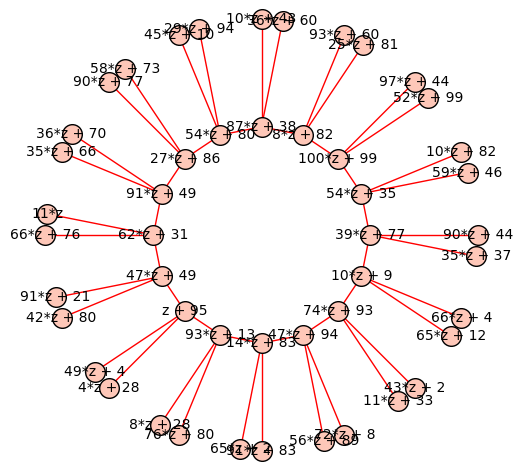
\includegraphics{./example_II.png}
    \caption{\label{fig:example_II} A 3-isogeny vulcano over $\F_{101^2} = \F_{101}[\alpha]$ that satisfies case II (in the plot have $z = \alpha$). Note that e.g. $(39\alpha + 77)^{101} = 62\alpha + 31$.}
\end{figure}

Further, when we consider the path $E = E_0 \to ... \to E_n = E^{(p)}$ on the crater, there are more or less two possibilities for the $\cdot^{(p)}$ conjugate path\footnote{Remember that $\cdot^{(p)}$ is functorial, hence we can also apply to isogenies $E_i \to E_{i + 1}$}.
\begin{itemize}
    \item It could be that the conjugate of $E_i \to E_{i + 1}$ is the dual of $E_{n - i - 1} \to E_{n - i}$, hence we just go the path $E \to ... \to E^{(p)}$ backwards.
    \item It could be that the conjugate of $E_i \to E_{i + 1}$ is $E_{n + i} \to E_{n + i + 1}$, where
    \begin{equation*}
        E_0, ..., E_n, E_{n + 1}, ..., E_{n + m} = E_0
    \end{equation*}
    is the cycle along the whole crater.
\end{itemize}
Both cases have interesting consequences:

\paragraph*{First case} The fact that the conjugate of $E_i \to E_{i + 1}$ is the dual of $E_{n - i - 1} \to E_{n - i}$ implies that $E_i^{(p)} = E_{n - i}$.
In particular, if $n$ is even, we find that $E_{n/2}$ is defined over $\F_p$.

Note that we have
\begin{prop}
    Let $E$ be an ordinary Elliptic Curve defined over a finite field of characteristic $p$.
    \begin{itemize}
        \item $\End(E)$ has an element of norm $p$ iff $j(E) \in \F_p$.
        \item $\End(E)$ has a nontrivial element (i.e. $\neq \pm p$) of norm $p^2$ iff $j(E) \in \F_{p^2}$. 
    \end{itemize}
\end{prop}
\begin{proof}
    The directions $\Leftarrow$ is clear, as the norm of the $q$-th power Frobenius endomorphism is $q$.

    For the direction $\Rightarrow$, assume there is an element $\alpha \in \End(E)$ with $N(\alpha) = p$.
    If $\alpha$ is inseparable (as isogeny), then we have that it factors through the $p$-th power Frobenius endomorphism $\pi$, and thus $\alpha = \lambda \circ \pi$ for an isomorphism $\lambda: E^{(p)} \to E$.
    Thus $j(E^{(p)}) = j(E)$.

    On the other hand, if $\alpha$ is separable, it must have kernel of size $p$, so $\ker(\alpha) = E[p]$ since $\#E[p] = p$ ($E$ is ordinary).
    Thus $\ker(\alpha) \subseteq \ker([p])$ and we see that $[p]$ factors through $\alpha$ as $[p] = \psi \circ \alpha$.
    Now have that $\deg(\psi) = p = p^2/\deg(\alpha)$ and clearly $\psi$ is inseparable.
    The claim follows as above.

    For the second point, assume $\alpha \in \End(E)$ has norm $N(\alpha) = p^2$ and $\alpha \neq \pm p$.
    If $\alpha$ is purely inseparable, we are done.
    If $\alpha$ is separable, its kernel must be $E[p^2]$ and so it factors through $[p^2]$.
    Since $[p^2]$ has inseparability degree $p^2$, we see that $[p^2] = \pi^2 \circ \alpha$ where $\pi$ is the $p$-th power Frobenius morphism.
    Since $\alpha$ is an endomorphism of $E$, find $\pi^2: E \to E$, thus $j(E) \in \F_{p^2}$.

    Finally, if $\alpha$ has inseparability degree $p$, then its kernel must be $E[p]$ and so $\alpha = \beta \circ \pi$ where $\beta: E^{(p)} \to E$ is separable with kernel $E^{(p)}[p]$.
    However, by the uniqueness of the separable isogeny with kernel $E^{(p)}[p]$, we know that (up to isomorphism) also $[p]$ is $\beta \circ \pi$.
    Thus $\alpha = \pm p$, a contradiction.
\end{proof}
In particular, it follows that either all or none of the curves on the crater of the vulcano have $j(E) \in \F_p$. 
\begin{prop}
    Let $[\b] \in \Cl(\O)$ where $\O = \End(E)$ for an ordinary Elliptic Curve $E/\F_{p^2}$ such that $[\b].E = E^{(p)}$.
    Then $[\b]^2 = [(1)]$.
\end{prop}
\begin{proof}
    We recall the definition of the class group action in the case $[\b].E^{(p)}$.
    For an ideal $\b' \leq \End(E^{(p)})$, have by definition
    \begin{equation*}
        [\b'].E^{(p)} = E^{(p)} / E^{(p)}[\b'] = E^{(p)} / \bigcap_{\beta \in \b'} \ker(\beta)
    \end{equation*}
    However, $\b$ is an ideal in $\End(E)$, which is only isomorphic to $\End(E^{(p)})$.
    Since $\End^0(E)$ is a quadratic imaginary number field, it has one nontrivial field automorphism, and thus the isomorphism $\End(E) \cong \End(E^{(p)})$ is not unique.
    But there is a unique canonical isomorphism, i.e. an isomorphism that is induced by an (equivalently any) isogeny $\phi: E \to E^{(p)}$ as
    \begin{equation*}
        \Phi_*: \End(E) \to \End(E^{(p)}), \quad \alpha \mapsto \frac 1 {\deg(\phi)} \ \phi \circ \alpha \circ \hat{\phi}
    \end{equation*}
    This is the isomorphism we use, i.e. we say
    \begin{equation*}
        E^{(p)}[\b] = E^{(p)}[\Phi_*(\b)] \quad \text{and} \quad [\b].E^{(p)} = [\Phi_*(\b)].E^{(p)} = E^{(p)}/E^{(p)}[\b]
    \end{equation*}

    Now let $\phi: E \to E/E[\b] = E^{(p)}$ be a separable isogeny with kernel $E[\b]$ (by choosing the representative $\b$ of $[\b] \in \Cl(\O)$ correspondingly, we can assume that).
    We have
    \begin{equation*}
        \ker(\phi^{(p)}) = E[\b]^{(p)} = \bigcap_{\beta \in \b} \ker(\beta)^{(p)} = \bigcap_{\beta \in \b} \ker(\beta^{(p)}) = \bigcap_{\beta \in \b^{(p)}} \ker(\beta)
    \end{equation*}
    Now note that the Frobenius isogeny $\pi: E \to E^{(p)}, \ P \mapsto P^{(p)}$ induces the canonical isomorphism $\End(E) \to \End(E^{(p)})$ and so the image of $\b$ under that isomorphism is $\b' = \b^{(p)} \leq \End(E^{(p)})$.
    Thus
    \begin{equation*}
        \bigcap_{\beta \in \b^{(p)}} \ker(\beta) = \bigcap_{\beta \in \b'} \ker(\beta) = E^{(p)}[\b'] = E^{(p)}[\b]
    \end{equation*}
    So by the uniqueness of the image curve for an isogeny with fixed kernel yields that $E = \mathrm{im}(\phi^{(p)}) = [\b].E^{(p)}$.
    Thus $[\b]^2.E = [\b].E^{(p)} = E$ and since the class group action is free, we see that $[\b]^2 = [(1)]$.
\end{proof}
From this we get the
\begin{figure}
    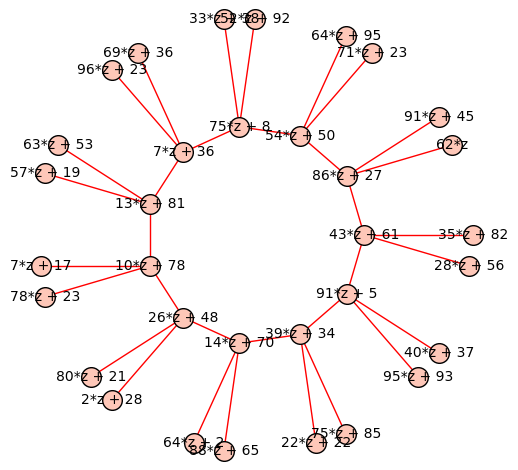
\includegraphics{./example_odd_crater.png}
    \caption{\label{fig:example_odd_crater} A 3-isogeny vulcano over $\F_{101^2} = \F_{101}[\alpha]$ that satisfies case III (in the plot have $z = \alpha$).}
\end{figure}
\begin{corollary}
    Assume that $E = E_0 \to E_1 \to ... \to E_n = E$ is the cycle once around the crater (and $j(E) \in \F_{p^2} \setminus \F_p$).
    If $E^{(p)} = E_i$ then $n$ is even and $i = n/2$, i.e. $E^{(p)}$ is on the other side of the crater\footnote{Note that this does not hold if $E, E^{(p)}$ are not in the same crater, see Figure~\ref{fig:example_odd_crater}.}.
\end{corollary}
\begin{proof}
    If $l$ does not split in $\O_\K$, then the crater has at most two elements and this is trivial.
    So assume $(l) = \l_1 \l_2$.
    It is known that then the action of $[\l_1]$ resp. $[\l_2]$ corresponds to walking around the crater in one direction resp. the other.
    So wlog $[\l_1].E_i = E_{i + 1}$.

    Now assume that $E^{(p)} = E_i$, so $[\b].E = E_i = [\l_1]^i.E$.
    Since the action is free, it follows that $[\b] = [\l_1]^i$
    By the previous theorem, we have now $[\l_1]^{2i} = [\b]^2 = [(1)]$ and so $[\l_1]^{2i}.E = E_{2i} = E$.
    Thus $i = n/2$ and the claim follows.
\end{proof}
In particular, the path between $E$ and $E^{(p)}$ is likely to have length $\omega(\log(p))$, since the crater is usually large.
This is displayed e.g. Figure~\ref{fig:example_II}.

\subsection{Case III}
\begin{figure}
    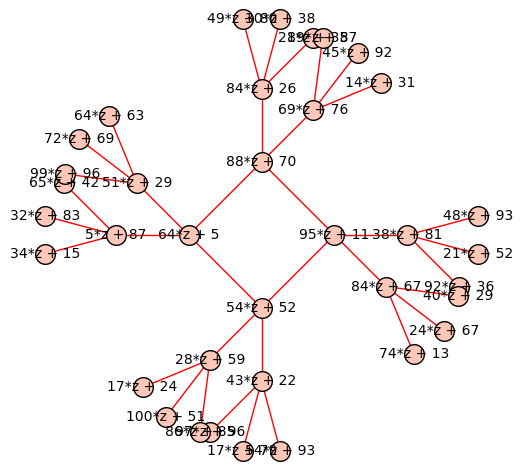
\includegraphics{./example_III.png}
    \caption{\label{fig:example_III} A 3-isogeny vulcano over $\F_{101^2} = \F_{101}[\alpha]$ that satisfies case III (in the plot have $z = \alpha$).}
\end{figure}
We give the example displayed in Figure~\ref{fig:example_III}.
Consider $E$ with $j(E) = 64\alpha + 5$.
Then $j(E^{(p)}) = j(E)^p = 37\alpha + 59$.
However, we have that $E$ lies on the crater, together with curve of j-invariants
\begin{equation*}
    88\alpha + 70, \ 54\alpha + 52, \ 95\alpha + 11
\end{equation*}
Hence there is no 3-isogeny path from $E$ to $E^{(p)}$.
Note that $[\O_\K : \Z[\pi]] = 2^2 \cdot 3^2$ but $[\O_\K : \End(E)] = 2^2$, which shows that $E$ lies on the crater.

Now we want to have a closer look onto the class group action in this case.
Have $d(\End(E)) = -320$, so $\K = \mathbb{Q}(\sqrt{-5})$ and $d(\O_\K) = -5$.
Hence, we have $\End(E) \cong \Z[4\sqrt{-5}]$ and $\O_\K \cong \Z[\sqrt{-5}]$.

Sage tells us that $h(\O_\K) = 2$ and $h(\End(E)) = 8$.
With this, we can already see that
\begin{equation*}
    64\alpha + 5, \ 88\alpha + 70, \ 54\alpha + 52, \ 95\alpha + 11
\end{equation*}
and
\begin{equation*}
    (64\alpha + 5)^p, \ (88\alpha + 70)^p, \ (54\alpha + 52)^p, \ (95\alpha + 11)^p
\end{equation*}
is the set of j-invariants of all Elliptic Curves with endomorphism ring $\cong \End(E)$.
On this set, $\Cl(\Z[4\sqrt{-5}])$ then acts freely and transitively.
Now it would be of course interesting to find out how $\Cl(\Z[4\sqrt{-5}])$ really looks like.

\section{Properties of the endomorphism ring vs the cases}
Let $E/\F_{p^2}$ be an ordinary Elliptic Curve and write $\O := \End(E), \K := \End(E) \otimes \mathbb{Q}$.
Let $\pi$ be the $q = p^2$-th power Frobenius endomorphism and let $t$ be the trace of Frobenius.
Assume $p \neq 2$.
\begin{lemma}
    Have $(p) = (p, \pi)(p, \pi - t)$.
\end{lemma}
\begin{proof}
    Have
    \begin{equation*}
        (p, \pi)(p, \pi - t) = (p^2, p\pi, p\pi - pt, \pi^2 - t\pi) = (p^2, pt, p\pi, -p^2) = (up^2 + vtp, ...) = (p)
    \end{equation*}
    where $up + vt = 1$ (note that $t \perp p$ since $E$ is ordinary).
\end{proof}
\begin{prop}
    Let $E/\F_{p^2}$ be an ordinary Elliptic Curve.
    Then $p = p_1 p_2$ in $\End(E)$.
\end{prop}

\section{Example - The ordinary endomorphism ring}
\begin{table}
    \begin{center}
        \begin{tabular}{c c c}
            $j(E)$ & $h(\End(E))$ & $[\O_\K : \Z[\phi]]$ \\
            \hline
            $\alpha$ & 36 & 6 \\
            $4\alpha + 99$ & 64 & 2
        \end{tabular}
    \end{center}
    \caption{\label{tab:class_numbers_of_endo_rings} Table of class numbers of $\End(E)$ for Elliptic Curves $E/\F_{101^2} = \F_{101}[\alpha]$.}
\end{table}
The information in this section is all known material - I just wanted to understand properly how one can compute the endomorphism ring, and what problems occur.

Consider the finite field
\begin{equation*}
    \F_q = \F_{37^2} = \F_{37} + \alpha \F_{37}
\end{equation*}
where $\alpha^2 + 33\alpha + 2 = 0$.
Further, consider the Elliptic Curve $E/\F_q$ with j-invariant $3\alpha$, given by
\begin{equation*}
    E: y^2 = x^3 + (15\alpha + 17)x + (5\alpha + 3)
\end{equation*}
Then we find that the $q$-th power Frobnenius endomorphism $\pi$ satisfies the minimal equation
\begin{equation*}
    \pi^2 + 47 \pi + 1369
\end{equation*}
and in particular, its trace is $-47$.
Hence, the number field $\K := \O \otimes \mathbb{Q}$ where $\O = \End(E)$ contains $\sqrt{47^2 - 4 \cdot 1369} = \sqrt{-3^3 \cdot 11^2}$.
We observe that $\K = \mathbb{Q}(\sqrt{-3})$ and has discriminant $-3$.
Furthermore the ring of integers is $\O_\K = \Z[\frac 1 2(1 + \sqrt{-3})]$.

Knowing the number field, we want to find the endomorphism ring.
First, observe that the Frobenius order $\Z[\pi]$ has conductor 33.
Now consider the endomorphism
\begin{equation*}
    \phi := 2\pi + 47
\end{equation*}
The advantage is that we can evaluate $\phi$ on points of $E$, but evaluating $\pi + 47/2$ is not so easy.
Clearly $[\Z[\pi] : \Z[\phi]] = 2$ and so $\Z[\phi]$ has conductor 66.

\subsection*{Torsion points}
In order to find whether $\phi/n \in \O$, we factor $66 = 2 \cdot 3 \cdot 11$ and compute the corresponding torsion groups.
This turns out to be quite difficult.

Assume $\F_{37^{12}} = \F_{37}[\beta]$ with
\begin{equation*}
    \mathrm{MiPo}_{\F_{37}}(\beta) = x^{12} + 4x^7 + 31x^6 + 10x^5 + 23x^4 + 18x^2 + 33x + 2
\end{equation*}
Then $E[2]$ is generated by
\begin{align*}
    P_1 &= (11\beta^{11} + 19\beta^{10} + \beta^9 + 27\beta^8 + 8\beta^7 + 16\beta^6 + 17\beta^5 + 32\beta^4 + 12\beta^3 + 14\beta^2 + 24\beta + 32 : 0 : 1) \\
    Q_1 &= (15\beta^{11} + 7\beta^{10} + 33\beta^9 + 11\beta^8 + 6\beta^7 + 12\beta^6 + 26\beta^5 + 7\beta^4 + 33\beta^3 + 25\beta^2 + 8\beta + 19 : 0 : 1)
\end{align*}
Further $E[3]$ is generated by
\begin{align*}
    P_2 &= (19\beta^{11} + 34\beta^{10} + 3\beta^9 + 29\beta^8 + 7\beta^7 + 3\beta^6 + 18\beta^5 + 21\beta^4 + 23\beta^3 + 30\beta^2 + 23\beta + 25 \\
    &: 6\beta^{11} + 25\beta^{10} + 4\beta^9 + 13\beta^8 + 10\beta^7 + 23\beta^6 + 20\beta^5 + 30\beta^4 + 24\beta^3 + 6\beta^2 + 17\beta + 5 : 1) \\
    Q_2 &= (31\beta^{11} + 24\beta^{10} + 35\beta^9 + 32\beta^8 + 2\beta^7 + 10\beta^6 + 23\beta^5 + 35\beta^4 + 22\beta^3 + 13\beta^2 + 12\beta + 12 \\
    &: 18\beta^{11} + 2\beta^{10} + 32\beta^9 + 26\beta^8 + 17\beta^7 + 5\beta^6 + 19\beta^5 + 31\beta^4 + 31\beta^3 + \beta^2 + 22\beta + 1 : 1)
\end{align*}

For $E[11]$ we must even go to the extension degree 110.
So assume $\F_{37^{220}} = \F_{37}[\gamma]$.
Then $E[11]$ is generated by $P_3$ and $Q_3$.
For the values of $\mathrm{MiPo}_{\F_{37}}(\gamma)$ and $P_3, Q_3$ see Section~\ref{sec:numerical_values}.

Now we can compute $\phi(P_1), \phi(Q_1), \phi(P_2), \phi(Q_2), \phi(P_3), \phi(Q_3)$ and see that none of them is zero.
Since $\deg(\phi) = [\O : \Z[\phi]] \divides [\O_\K : \Z[\phi]] = 2 \cdot 3 \cdot 11$, we see that the kernel of $\phi$ is trivial.
Thus no $\phi/n$ is contained in $\O$.
Therefore we see that
\begin{equation*}
    \O \cap \Z[\sqrt{D}] = \Z[\phi]
\end{equation*}
The inclusion $\supseteq$ is clear, and for the other direction, note that $\O \cap \Z[\sqrt{D}] = \Z + t\sqrt{D}\Z$ and $\Z[\phi] = \Z + s\sqrt{D}\Z$.
Since $\Z[\phi] \subseteq \O \cap \Z[\phi]$ find thus $t \divides s$.
Now observe that by choice of $\phi$, have $\phi^2 \in \Z$ and so $\phi = s\sqrt{D}$.
However, $\phi/\frac s t = t \sqrt{D} \in \O$.
By the above, it follows that $\frac s t = 1$, i.e. $s = t$.

\subsection*{The index $[\O : \Z[\phi]]$}
From the consideration of the torsion points, we see that $\O \cap \Z[\sqrt{D}] = \Z[\phi]$.
However, since $[\O_\K : \Z[\sqrt{D}]] \leq 2$, we deduce that $[\O : \Z[\phi]] \leq 2$ and so
\begin{equation*}
    \O = \Z[\pi]
\end{equation*}

\section{$P_3$ and $Q_3$}
\label{sec:numerical_values}
The minimal polynomial of $\gamma$ is
\begin{lstlisting}
    x^220 + 31*x^219 + 13*x^218 + 21*x^217 + 23*x^216 + 9*x^215 
    + 2*x^214 + 35*x^212 + 10*x^211 + 29*x^210 + 25*x^209 + 20*x^208 
    + 17*x^207 + 30*x^206 + 5*x^205 + 15*x^204 + 11*x^203 + 10*x^202 
    + 11*x^201 + 32*x^200 + 5*x^199 + 28*x^198 + 7*x^197 + 13*x^196 
    + 10*x^195 + 32*x^194 + 17*x^193 + 19*x^192 + 36*x^191 
    + 17*x^190 + 31*x^189 + 14*x^188 + 6*x^187 + 30*x^186 + 8*x^185 
    + 22*x^184 + 2*x^183 + 9*x^182 + 11*x^181 + 6*x^180 + 23*x^179 
    + 14*x^178 + 36*x^177 + 16*x^176 + 34*x^175 + 14*x^174 
    + 33*x^173 + 14*x^172 + 7*x^171 + 36*x^170 + 18*x^169 + 27*x^168 
    + 5*x^167 + 31*x^166 + 6*x^165 + 15*x^164 + 14*x^163 + 17*x^162 
    + 7*x^161 + 16*x^160 + 6*x^159 + 29*x^158 + 11*x^157 + 8*x^156 
    + 15*x^155 + 20*x^154 + 17*x^153 + 7*x^152 + 8*x^151 + 6*x^150 
    + 12*x^149 + 36*x^148 + 7*x^147 + 3*x^146 + 25*x^145 + 13*x^144 
    + 6*x^143 + 17*x^142 + 22*x^141 + 9*x^140 + 18*x^139 + 36*x^138 
    + x^137 + 6*x^136 + 36*x^135 + 33*x^134 + 32*x^133 + 35*x^132 
    + 33*x^131 + 7*x^130 + 3*x^129 + 7*x^128 + 20*x^127 + 31*x^126 
    + 26*x^125 + 6*x^124 + 9*x^123 + 10*x^122 + 25*x^121 + 33*x^120 
    + 33*x^119 + 30*x^118 + 34*x^117 + 22*x^116 + 8*x^115 + 10*x^114 
    + 36*x^113 + 26*x^112 + 8*x^111 + 33*x^110 + 30*x^109 + 11*x^108 
    + 14*x^107 + 22*x^106 + 26*x^105 + 11*x^104 + 35*x^103 
    + 34*x^102 + 33*x^101 + 27*x^100 + 14*x^99 + 31*x^98 + 24*x^97 
    + x^96 + 6*x^95 + 36*x^93 + 32*x^92 + 18*x^91 + 36*x^90 + 3*x^89 
    + 22*x^88 + 36*x^87 + 6*x^86 + 20*x^85 + 25*x^84 + 8*x^82 
    + 34*x^81 + 7*x^80 + 25*x^79 + 21*x^78 + 17*x^77 + 29*x^76 
    + 5*x^75 + 19*x^74 + 19*x^73 + 8*x^72 + 8*x^71 + 26*x^70 
    + 7*x^69 + 27*x^68 + 10*x^67 + 31*x^66 + 4*x^65 + 29*x^64 
    + 36*x^62 + 3*x^61 + 27*x^60 + 13*x^59 + 23*x^58 + 33*x^57 
    + 14*x^56 + 19*x^55 + 12*x^54 + 20*x^53 + 32*x^52 + 18*x^51 
    + 20*x^49 + 20*x^48 + x^47 + 17*x^46 + 16*x^45 + 4*x^44 
    + 12*x^43 + 7*x^42 + 34*x^41 + 9*x^40 + 16*x^39 + 10*x^38 
    + 25*x^37 + 10*x^36 + 10*x^35 + 28*x^34 + 33*x^33 + 22*x^32 
    + 24*x^31 + 33*x^30 + 6*x^29 + 8*x^28 + 8*x^27 + 16*x^26 
    + 31*x^25 + 7*x^24 + 26*x^23 + 36*x^22 + 29*x^21 + 36*x^20 
    + 7*x^19 + x^18 + 26*x^17 + 18*x^16 + 23*x^15 + 10*x^14 
    + 4*x^13 + x^12 + 24*x^11 + 25*x^10 + 34*x^9 + 33*x^8 
    + 33*x^7 + 8*x^6 + 12*x^5 + x^4 + 15*x^3 + 27*x^2 + 9*x + 2
\end{lstlisting}
$P_3$ is given by
\begin{lstlisting}
    (23*z220^219 + 5*z220^218 + 26*z220^217 + 27*z220^216 
    + 26*z220^215 + 12*z220^214 + 11*z220^213 + 10*z220^212 
    + 29*z220^211 + 9*z220^210 + 16*z220^209 + 24*z220^208 
    + 18*z220^207 + 11*z220^206 + 11*z220^205 + 6*z220^204 
    + 24*z220^203 + 3*z220^202 + 34*z220^201 + 18*z220^200 
    + 17*z220^199 + 9*z220^198 + 26*z220^197 + 2*z220^196 
    + 31*z220^195 + 7*z220^194 + 15*z220^193 + 11*z220^192 
    + 15*z220^191 + 28*z220^190 + 13*z220^189 + 6*z220^188 
    + 7*z220^187 + 28*z220^186 + 9*z220^185 + 9*z220^184 
    + 7*z220^183 + 27*z220^182 + 36*z220^181 + 35*z220^180 
    + 30*z220^179 + 32*z220^178 + 16*z220^177 + 15*z220^176 
    + 16*z220^175 + 9*z220^174 + 21*z220^173 + 6*z220^172 
    + 15*z220^171 + 3*z220^170 + 25*z220^169 + 23*z220^168 
    + z220^167 + 8*z220^166 + 34*z220^165 + 14*z220^164 
    + 12*z220^163 + 20*z220^162 + 4*z220^161 + 9*z220^160 
    + z220^159 + 25*z220^158 + 16*z220^157 + z220^156 
    + 21*z220^155 + 10*z220^154 + 7*z220^153 + 13*z220^152 
    + 32*z220^151 + 31*z220^150 + 17*z220^148 + 24*z220^147 
    + 26*z220^146 + 28*z220^145 + 27*z220^144 + 4*z220^143 
    + 5*z220^142 + 14*z220^141 + 26*z220^140 + 10*z220^139 
    + 14*z220^138 + 19*z220^137 + 20*z220^136 + 18*z220^135 
    + 16*z220^134 + 11*z220^133 + 23*z220^132 + 35*z220^131 
    + 22*z220^130 + 31*z220^129 + 34*z220^128 + 17*z220^127 
    + z220^126 + 15*z220^125 + 2*z220^124 + 22*z220^123 
    + 27*z220^122 + 6*z220^121 + 10*z220^120 + 7*z220^119 
    + 4*z220^118 + 26*z220^117 + z220^116 + 32*z220^115 
    + 29*z220^114 + 32*z220^113 + 18*z220^112 + 3*z220^111 
    + 28*z220^110 + 20*z220^109 + 17*z220^108 + 17*z220^107 
    + 32*z220^106 + 32*z220^105 + 26*z220^104 + 24*z220^103 
    + 17*z220^102 + 8*z220^101 + 3*z220^100 + 2*z220^99 
    + 16*z220^98 + 29*z220^97 + 19*z220^96 + 27*z220^95 
    + 4*z220^94 + 29*z220^93 + 24*z220^92 + 19*z220^91 
    + 2*z220^90 + 2*z220^89 + 32*z220^88 + 23*z220^87 
    + 32*z220^86 + 15*z220^85 + 24*z220^84 + 36*z220^83 
    + 29*z220^82 + 18*z220^81 + 2*z220^80 + z220^79 
    + 33*z220^78 + 34*z220^77 + 4*z220^76 + 11*z220^75 
    + 21*z220^74 + 15*z220^73 + 10*z220^72 + 24*z220^71 
    + 22*z220^70 + 22*z220^69 + 31*z220^68 + 32*z220^67 
    + 28*z220^66 + z220^65 + 17*z220^64 + 13*z220^63 
    + 32*z220^62 + 20*z220^61 + 32*z220^60 + 21*z220^59 
    + 34*z220^58 + 11*z220^57 + 29*z220^56 + 12*z220^55 
    + 22*z220^54 + 11*z220^53 + 36*z220^52 + 35*z220^51 
    + 19*z220^50 + 35*z220^49 + 8*z220^48 + 16*z220^47 
    + 16*z220^46 + 27*z220^45 + 32*z220^44 + 12*z220^43 
    + 15*z220^42 + 6*z220^41 + 36*z220^40 + 27*z220^39 
    + 17*z220^38 + 20*z220^37 + 33*z220^36 + 34*z220^35 
    + 34*z220^34 + 3*z220^33 + 12*z220^32 + 12*z220^31 
    + 12*z220^30 + 5*z220^29 + 10*z220^28 + 13*z220^27 
    + 36*z220^26 + 16*z220^25 + 16*z220^24 + 15*z220^23 
    + 36*z220^22 + 18*z220^21 + 13*z220^20 + 26*z220^19 
    + 25*z220^18 + 21*z220^17 + 35*z220^16 + 3*z220^14 
    + 31*z220^13 + 8*z220^12 + 7*z220^11 + 10*z220^10 
    + 10*z220^9 + 6*z220^8 + 5*z220^7 + 33*z220^6 
    + 6*z220^5 + 4*z220^4 + 31*z220^3 + 27*z220^2 + 27*z220 + 14 
    
    : 8*z220^219 + 17*z220^218 + 27*z220^217 + 14*z220^216 
    + 6*z220^215 + 19*z220^214 + 18*z220^213 + 6*z220^212 
    + 30*z220^211 + 24*z220^210 + 33*z220^209 + 19*z220^208 
    + 27*z220^207 + 16*z220^206 + 24*z220^205 + 3*z220^204 
    + 4*z220^203 + 25*z220^202 + 29*z220^201 + 31*z220^200 
    + 23*z220^199 + 7*z220^198 + 28*z220^197 + 4*z220^196 
    + 26*z220^195 + 36*z220^194 + 18*z220^193 + 24*z220^192 
    + 29*z220^191 + 25*z220^190 + 23*z220^189 + 14*z220^188 
    + 33*z220^187 + 19*z220^186 + 14*z220^184 + 21*z220^183 
    + 10*z220^182 + 13*z220^181 + 21*z220^180 + 24*z220^179 
    + 33*z220^178 + 19*z220^177 + 7*z220^176 + 36*z220^175 
    + 30*z220^174 + 34*z220^173 + 27*z220^172 + 3*z220^171 
    + 34*z220^170 + 5*z220^169 + 36*z220^168 + 19*z220^167 
    + 27*z220^166 + 14*z220^165 + 10*z220^164 + 2*z220^163 
    + 31*z220^162 + 22*z220^161 + 7*z220^160 + 14*z220^159 
    + 5*z220^158 + 3*z220^157 + 22*z220^156 + 32*z220^155 
    + 21*z220^154 + 17*z220^153 + 34*z220^152 + 9*z220^151 
    + 33*z220^150 + 32*z220^149 + 24*z220^148 + 16*z220^147 
    + 19*z220^146 + 6*z220^145 + 26*z220^144 + 24*z220^143 
    + 34*z220^141 + 25*z220^140 + 17*z220^139 + 25*z220^138 
    + 19*z220^137 + 36*z220^136 + 7*z220^134 + 32*z220^133 
    + 24*z220^132 + 6*z220^131 + 12*z220^130 + 30*z220^129 
    + 35*z220^128 + 13*z220^127 + 29*z220^126 + 2*z220^125 
    + 24*z220^124 + 36*z220^123 + 34*z220^122 + 2*z220^121 
    + 33*z220^120 + 10*z220^119 + 33*z220^118 + 2*z220^117 
    + 17*z220^116 + 33*z220^115 + 14*z220^114 + 22*z220^113
    + 27*z220^112 + 20*z220^111 + 23*z220^110 + 34*z220^109 
    + 6*z220^108 + 33*z220^107 + 14*z220^106 + 28*z220^105 
    + 29*z220^104 + 36*z220^103 + 22*z220^102 + 35*z220^101 
    + 8*z220^100 + 10*z220^99 + 10*z220^98 + 16*z220^97 
    + 19*z220^96 + 17*z220^95 + 21*z220^94 + 13*z220^93 
    + 24*z220^92 + 36*z220^91 + 25*z220^90 + 25*z220^89 
    + 22*z220^88 + 27*z220^87 + 28*z220^86 + 11*z220^85 
    + 3*z220^84 + 14*z220^82 + 31*z220^81 + 7*z220^80 
    + 33*z220^79 + 33*z220^78 + 2*z220^77 + 15*z220^76 
    + 17*z220^75 + 32*z220^74 + 4*z220^73 + 18*z220^72 
    + 10*z220^71 + 34*z220^70 + 9*z220^69 + 3*z220^68 
    + 20*z220^67 + 33*z220^66 + 23*z220^65 + 5*z220^64 
    + 20*z220^63 + 36*z220^62 + 29*z220^61 + 2*z220^60 
    + 25*z220^59 + 14*z220^58 + 16*z220^57 + 31*z220^56 
    + 22*z220^55 + 31*z220^54 + 33*z220^53 + 19*z220^52 
    + 22*z220^51 + 23*z220^50 + 36*z220^49 + 11*z220^48 
    + 15*z220^47 + 15*z220^46 + 35*z220^45 + 7*z220^44 
    + 27*z220^43 + 28*z220^42 + 15*z220^41 + 31*z220^40 
    + 12*z220^39 + 19*z220^38 + 21*z220^37 + 18*z220^36 
    + 3*z220^35 + 36*z220^33 + z220^32 + 35*z220^31 
    + 21*z220^30 + 2*z220^29 + 13*z220^28 + 19*z220^27 
    + 6*z220^26 + 22*z220^24 + 26*z220^23 + 9*z220^22 
    + 7*z220^21 + 31*z220^20 + 31*z220^19 + 9*z220^18 
    + 23*z220^17 + 23*z220^16 + 6*z220^15 + 27*z220^14 
    + 36*z220^13 + 4*z220^12 + 26*z220^11 + 30*z220^10 
    + 9*z220^9 + 8*z220^8 + 15*z220^7 + 26*z220^6 
    + 17*z220^5 + 29*z220^4 + 24*z220^3 + 8*z220^2 
    + 29*z220 : 1)
\end{lstlisting}
$Q_3$ is given by
\begin{lstlisting}
    (35*z220^219 + 22*z220^218 + 36*z220^216 + 24*z220^215 
    + 19*z220^214 + 32*z220^213 + 13*z220^212 + 19*z220^211 
    + 3*z220^210 + 36*z220^209 + 29*z220^208 + 35*z220^206 
    + 31*z220^205 + 32*z220^204 + 23*z220^203 + 21*z220^202 
    + 10*z220^201 + 32*z220^200 + 32*z220^199 + 21*z220^198 
    + 16*z220^197 + 23*z220^196 + 32*z220^195 + 12*z220^194 
    + 9*z220^193 + 35*z220^192 + 8*z220^191 + 19*z220^190 
    + 33*z220^189 + 13*z220^188 + 11*z220^187 + 35*z220^186 
    + 25*z220^185 + 28*z220^184 + 5*z220^183 + 7*z220^182 
    + 24*z220^181 + 35*z220^180 + 33*z220^179 + 18*z220^178 
    + 5*z220^177 + 31*z220^176 + 18*z220^175 + 30*z220^174 
    + 27*z220^173 + 3*z220^172 + 8*z220^171 + 24*z220^170 
    + 14*z220^169 + 2*z220^168 + 16*z220^167 + 14*z220^166 
    + 18*z220^165 + 22*z220^164 + 32*z220^163 + 28*z220^162 
    + 7*z220^161 + 19*z220^160 + 3*z220^159 + 14*z220^158 
    + 27*z220^157 + 35*z220^156 + 8*z220^155 + 25*z220^154 
    + 11*z220^153 + 19*z220^152 + 21*z220^151 + 10*z220^150 
    + 2*z220^149 + 4*z220^148 + 4*z220^147 + 31*z220^146 
    + 26*z220^145 + 17*z220^143 + 14*z220^142 + 12*z220^141 
    + 17*z220^140 + 22*z220^139 + 30*z220^138 + 30*z220^137 
    + 15*z220^136 + 16*z220^135 + 25*z220^134 + 8*z220^133 
    + 28*z220^132 + 5*z220^131 + 14*z220^130 + 26*z220^129 
    + 13*z220^128 + 10*z220^127 + 13*z220^126 + 10*z220^125 
    + 17*z220^124 + 33*z220^123 + 9*z220^122 + 9*z220^121 
    + 10*z220^120 + 12*z220^119 + 4*z220^118 + 6*z220^117 
    + 33*z220^116 + 21*z220^115 + 14*z220^114 + 33*z220^113 
    + 11*z220^112 + 4*z220^111 + 3*z220^110 + 3*z220^109 
    + 3*z220^108 + 3*z220^107 + 27*z220^106 + 8*z220^105 
    + 25*z220^104 + 10*z220^103 + 24*z220^102 + 2*z220^101 
    + 12*z220^100 + 35*z220^99 + 30*z220^98 + 14*z220^97 
    + 8*z220^96 + 16*z220^95 + 24*z220^94 + 23*z220^93 
    + 34*z220^91 + 3*z220^90 + 13*z220^89 + 10*z220^88 
    + 20*z220^87 + 14*z220^86 + 9*z220^85 + 36*z220^84 
    + 33*z220^83 + 12*z220^82 + 20*z220^81 + 5*z220^80 
    + 27*z220^79 + 27*z220^78 + 9*z220^77 + 23*z220^76 
    + 4*z220^75 + 26*z220^74 + 8*z220^73 + 11*z220^72 
    + 25*z220^71 + 35*z220^70 + 19*z220^69 + 36*z220^68 
    + 35*z220^67 + 24*z220^66 + 8*z220^65 + 32*z220^64 
    + 10*z220^63 + 3*z220^62 + 18*z220^61 + 35*z220^60 
    + 17*z220^59 + 30*z220^58 + 2*z220^57 + 25*z220^56 
    + 7*z220^55 + 20*z220^54 + 27*z220^53 + z220^52 
    + 10*z220^51 + 2*z220^50 + 18*z220^49 + 30*z220^48 
    + 32*z220^47 + 20*z220^46 + 4*z220^45 + 16*z220^43 
    + 16*z220^42 + 11*z220^41 + 8*z220^40 + 12*z220^39 
    + 15*z220^38 + 25*z220^37 + 33*z220^36 + 4*z220^35 
    + 11*z220^34 + 6*z220^33 + 7*z220^32 + 32*z220^31 
    + 19*z220^30 + 19*z220^29 + 16*z220^28 + 10*z220^27 
    + 7*z220^26 + 10*z220^25 + 33*z220^24 + 25*z220^23 
    + 21*z220^22 + 35*z220^21 + 15*z220^20 + z220^19 
    + 19*z220^18 + 16*z220^17 + 10*z220^16 + 18*z220^15 
    + 17*z220^14 + 2*z220^13 + 35*z220^12 + 30*z220^11 
    + 17*z220^10 + 30*z220^9 + 26*z220^8 + 9*z220^7 
    + 34*z220^6 + 4*z220^5 + 12*z220^4 + 16*z220^3 
    + 27*z220^2 + 12*z220 + 36 
    
    : 21*z220^219 + 24*z220^218 
    + 33*z220^217 + 31*z220^216 + 29*z220^215 + 16*z220^214 
    + 26*z220^213 + 7*z220^212 + 15*z220^211 + 9*z220^210 
    + 19*z220^209 + 18*z220^208 + 16*z220^207 + 23*z220^206 
    + 27*z220^205 + 16*z220^204 + 5*z220^203 + 10*z220^202 
    + 2*z220^201 + 19*z220^200 + 19*z220^199 + 8*z220^198 
    + 30*z220^197 + 9*z220^196 + 27*z220^195 + 7*z220^194 
    + 20*z220^193 + 8*z220^192 + 29*z220^191 + 10*z220^190 
    + 32*z220^189 + 9*z220^188 + 4*z220^187 + 31*z220^186 
    + 8*z220^185 + 4*z220^184 + 8*z220^183 + 11*z220^182 
    + 13*z220^181 + 5*z220^180 + 29*z220^179 + 13*z220^178 
    + 20*z220^177 + 9*z220^176 + 3*z220^175 + 32*z220^174 
    + 3*z220^173 + 25*z220^172 + 33*z220^171 + 36*z220^170 
    + 11*z220^169 + 22*z220^168 + 18*z220^167 + 7*z220^166 
    + 4*z220^165 + 9*z220^164 + 33*z220^163 + 33*z220^162 
    + 18*z220^161 + 3*z220^160 + 35*z220^159 + 31*z220^158 
    + 20*z220^157 + 28*z220^155 + 33*z220^154 + 30*z220^153 
    + 28*z220^152 + 18*z220^151 + z220^150 + 34*z220^149 
    + 16*z220^148 + 23*z220^147 + 30*z220^146 + 3*z220^144 
    + 28*z220^143 + 8*z220^142 + 35*z220^140 + 11*z220^139 
    + 16*z220^138 + 20*z220^137 + 31*z220^136 + 11*z220^135 
    + 24*z220^134 + 29*z220^133 + 29*z220^132 + 8*z220^131 
    + 25*z220^130 + 11*z220^129 + 35*z220^128 + 36*z220^127 
    + 33*z220^126 + 18*z220^125 + 8*z220^124 + 9*z220^123 
    + 31*z220^122 + 29*z220^121 + 7*z220^120 + 4*z220^119 
    + 3*z220^118 + 13*z220^117 + 35*z220^116 + 17*z220^115 
    + 6*z220^114 + 3*z220^113 + 13*z220^112 + 5*z220^111 
    + 31*z220^110 + 32*z220^109 + 17*z220^108 + 28*z220^107 
    + 21*z220^106 + 14*z220^105 + 25*z220^104 + 17*z220^103 
    + 33*z220^102 + 19*z220^101 + 4*z220^100 + 2*z220^99 
    + 7*z220^98 + 34*z220^97 + 15*z220^96 + 7*z220^95 
    + 34*z220^94 + 22*z220^93 + 22*z220^92 + 11*z220^91 
    + 33*z220^90 + 32*z220^89 + 19*z220^88 + 21*z220^87 
    + 23*z220^86 + 34*z220^85 + 35*z220^84 + 23*z220^83 
    + 27*z220^82 + 25*z220^81 + 26*z220^80 + 2*z220^79 
    + 33*z220^78 + 32*z220^77 + 8*z220^76 + 32*z220^75 
    + 15*z220^74 + 17*z220^73 + 31*z220^72 + 7*z220^71 
    + 8*z220^70 + 8*z220^69 + 22*z220^68 + 7*z220^67 
    + 14*z220^66 + 15*z220^65 + 26*z220^64 + 26*z220^63 
    + 35*z220^62 + 19*z220^61 + 18*z220^60 + 22*z220^59 
    + 25*z220^57 + 4*z220^56 + 5*z220^55 + 4*z220^54 
    + 20*z220^53 + 32*z220^52 + 17*z220^51 + 14*z220^50 
    + 31*z220^49 + 9*z220^48 + 30*z220^47 + 20*z220^46 
    + 7*z220^45 + 16*z220^43 + 23*z220^42 + 12*z220^41 
    + 21*z220^40 + 14*z220^39 + 8*z220^38 + 14*z220^37 
    + 35*z220^36 + 14*z220^35 + 22*z220^34 + 8*z220^33 
    + z220^32 + 24*z220^31 + 21*z220^30 + 33*z220^29 
    + 21*z220^28 + 22*z220^26 + 33*z220^25 + 13*z220^24 
    + 13*z220^23 + 5*z220^22 + 35*z220^21 + 3*z220^20 
    + 31*z220^19 + 13*z220^18 + 33*z220^17 + 30*z220^16 
    + 16*z220^15 + 30*z220^14 + 16*z220^13 + 11*z220^12 
    + 35*z220^11 + 22*z220^10 + 11*z220^9 + 8*z220^8 
    + z220^7 + 25*z220^6 + 8*z220^5 + 27*z220^4 + z220^3 
    + 29*z220^2 + 34*z220 + 29 : 1)
\end{lstlisting}
\end{document}